\section{Grafi $P(R)$ za vse energijske pasove}
Kot samo ime sugestira, so grafi narejeni na podoben način kot v poglavju \ref{sec:1},
s to razliko, da ne ločujemo grafov po energiskih pasovih.
\begin{figure}[h]
    \begin{center}
        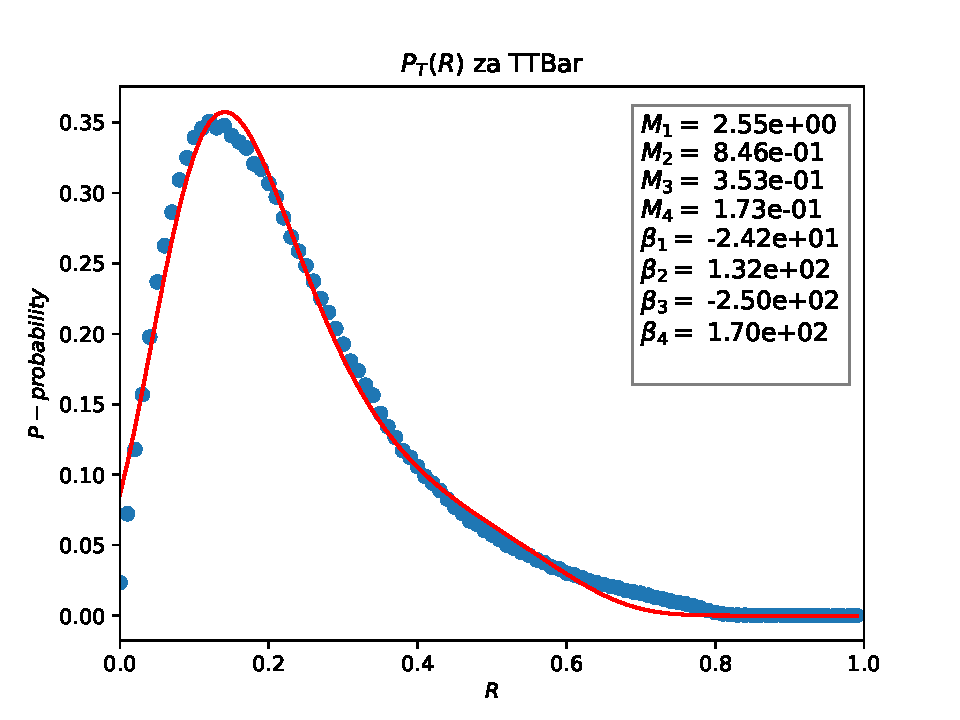
\includegraphics[width=13cm]{sections/section5/figures/pt_R-TTBar.pdf}
        \caption{Graf $P(R)$, s fitano funkcijo oblike $A \cdot \prod_i e^{\beta_i}$}
        \label{slika 7}
    \end{center}
\end{figure}
\\
Na graf sem še fital funkcijo oblike:
\begin{equation}
    f(x) = A \cdot \prod_i e^{\beta_i}
\end{equation}
Fitani so bili parametri $A$ in $\beta_i$. V levem zgornjem okvirčku so še izračunani momenti.
Podobno sem risal grafe funkcije $R^2$.
Koda je shranjena v \verb|MAIN/functions.py|, grafi pa v \verb|MAIN/pdfs|. Vsak graf pripada različni datoteki
in zato so shranjeni na način, ki sam po sebi pove, kaj predstavlja. Podatki so bili vzeti iz vseh oblik istih datotek.
Kot primer: \verb|TTBarLep_100.root TTBarLep_101.root ...|
\newpage\noindent
\begin{figure}[h]
    \begin{center}
        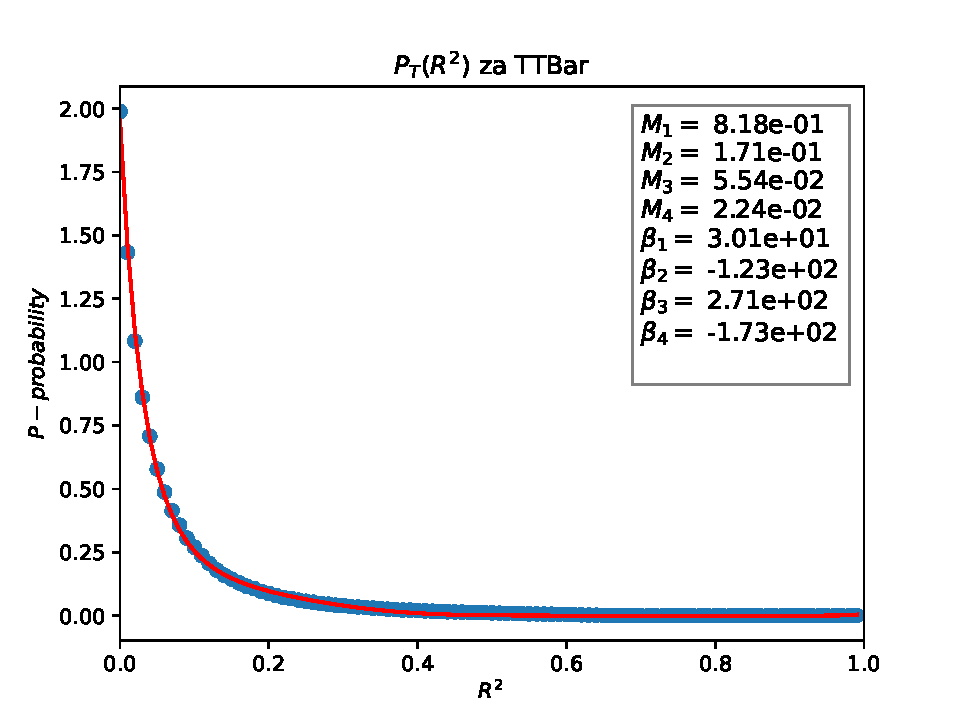
\includegraphics[width=13cm]{sections/section5/figures/pt_R2-TTBar.pdf}
        \caption{Graf $P(R^2)$, s fitano funkcijo oblike $A \cdot \prod_i e^{\beta_i}$}
        \label{slika 8}
    \end{center}
\end{figure}